\documentclass{beamer}
\usepackage{graphicx}
\usepackage{hyperref}
\usepackage{caption}
\usepackage{amsmath}
\usepackage{listings}
\usepackage{xcolor}

\setlength{\abovecaptionskip}{5pt}
\usetheme{metropolis}

% Personalizzazione dei colori
\definecolor{verdeScuro}{RGB}{0, 100, 0}
\setbeamercolor{frametitle}{bg=verdeScuro, fg=white}
\setbeamercolor{title}{bg=verdeScuro, fg=verdeScuro}
\setbeamercolor{footline}{bg=verdeScuro, fg=white}
\setbeamercolor{background canvas}{bg=white}
\setbeamercolor{title in head/foot}{fg=white, bg=verdeScuro}

% Imposta il font predefinito su Helvetica
\renewcommand{\familydefault}{\sfdefault}

% Stile per il codice
\lstset{
    basicstyle=\ttfamily\footnotesize,
    keywordstyle=\color{verdeScuro}\bfseries,
    commentstyle=\color{gray},
    stringstyle=\color{red},
    frame=single,
    breaklines=true,
    columns=fullflexible,
    language=R
}

\title{\textbf{\textcolor{verdeScuro}{Analisi Incendi Australia 2019-2024}}}
\subtitle{Monitoraggio della foresta australiana colpita dagli incendi tra il 2019 e il 2024}
\author{Martina Neri}
%\date{}

\begin{document}

\maketitle

\begin{frame}
\frametitle{Outline}
\tableofcontents
\end{frame}

\section{Introduzione}

\begin{frame}{\textbf{Introduzione}}
\textbf{Titolo:} Analisi Incendi in Australia (2019-2020-2024)
\newline
\newline
\textbf{Obiettivo:} Esaminare gli effetti degli incendi forestali del 2019 in Australia sull'ambiente tramite immagini satellitari.
\newline
\newline
\textbf{Approccio:} Confronto tra immagini pre e post incendio e analisi temporale degli indici spettrali e della Land cover.
\end{frame}

\section{Dati e Software Utilizzati}

\begin{frame}{\textbf{Dati e Software Utilizzati}}
\textbf{Dataset:} Immagini satellitari di tre date chiave (2019, 2020, 2024).
\newline
\newline
\textbf{Software:} R con i pacchetti \texttt{raster}, \texttt{ggplot2}, \texttt{viridis}.
\newline
\newline
\textbf{Indici Analizzati:}
\begin{itemize}
    \item DVI (Difference Vegetation Index)
    \item NDVI (Normalized Difference Vegetation Index)
\end{itemize}
\newline
\textbf{Strumenti di Analisi:}
\begin{itemize}
    \item PCA (Analisi delle Componenti Principali)
    \item Classificazione Land Cover (K-Means)
\end{itemize}
\end{frame}

\section{Caricamento e Visualizzazione dei Dati}

\begin{frame}[fragile]{\textbf{Caricamento e Visualizzazione dei Dati}}
\textbf{Impostazione della working directory:}
\begin{lstlisting}
setwd("C:/lab/Esame_telerilevamento/prova")
\end{lstlisting}

\textbf{Importazione delle immagini:}
\begin{lstlisting}
rlist_2019 <- list.files(pattern = "2019-02-22")
import_2019 <- lapply(rlist_2019, raster)
img_2019 <- stack(import_2019)
\end{lstlisting}

\textbf{Visualizzazione delle immagini:}
\begin{lstlisting}
par(mfrow = c(1, 2))
plotRGB(img_2019, 3, 2, 1, stretch = "lin") #True color
plotRGB(img_2019, 4, 3, 2, stretch = "lin") #NIR
\end{lstlisting}
Simile per 2020 e 2024.
\end{frame}

\section{Analisi degli Indici Spettrali}

\begin{frame}[fragile]{\textbf{Analisi degli Indici Spettrali}}
\textbf{DVI (Difference Vegetation Index):}
\begin{lstlisting}
# Formula
DVI_2019 <- img_2019[[4]] - img_2019[[3]]
DVI_2020 <- img_2020[[4]] - img_2020[[3]]
DVI_2024 <- img_2024[[4]] - img_2024[[3]]

# Differenze tra anni
DVI_diff_2020 <- DVI_2020 - DVI_2019 #danni dati dall'incendio
DVI_diff_2024 <- DVI_2024 - DVI_2020 #ripristino vegetazione

# Visualizzazione
par(mfrow = c(1, 3))
plot(DVI_2019, col = viridis(10), main = "DVI 2019")
plot(DVI_2020, col = viridis(10), main = "DVI 2020")
plot(DVI_2024, col = viridis(10), main = "DVI 2024")
\end{lstlisting}
\end{frame}

\begin{frame}{\textbf{Immagini DVI}}
\begin{columns}
    \column{1\textwidth}
    \centering
    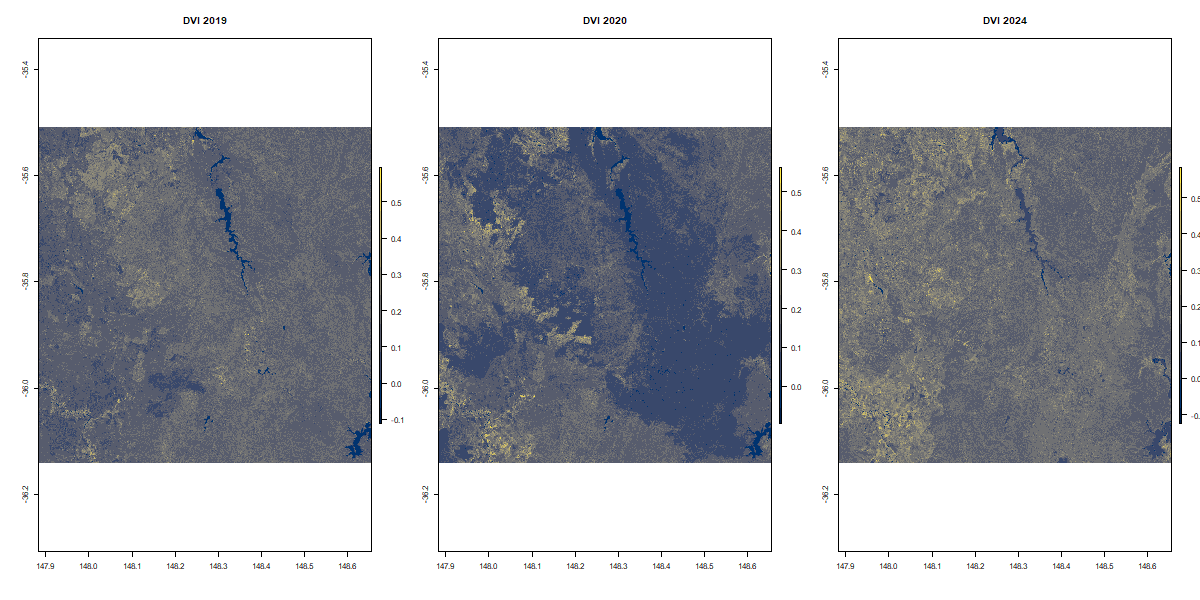
\includegraphics[width=\textwidth]{DVI.png}
\end{columns}
\end{frame}

\begin{frame}[fragile]{\textbf{Indice NDVI}}
\textbf{NDVI (Normalized Difference Vegetation Index):}
\begin{lstlisting}
# Formula
NDVI_2019 <- DVI_2019 / (img_2019[[4]] + img_2019[[3]])
NDVI_2020 <- DVI_2020 / (img_2020[[4]] + img_2020[[3]])
NDVI_2024 <- DVI_2024 / (img_2024[[4]] + img_2024[[3]])

# Cambiamenti temporali
NDVI_diff_2020 <- NDVI_2020 - NDVI_2019 #danni dati dall'incendio
NDVI_diff_2024 <- NDVI_2024 - NDVI_2020 #ripristino vegetazione

# Visualizzazione
par(mfrow = c(1, 3))
plot(NDVI_2019, col = viridis(10), main = "NDVI 2019")
plot(NDVI_2020, col = viridis(10), main = "NDVI 2020")
plot(NDVI_2024, col = viridis(10), main = "NDVI 2024")
\end{lstlisting}
\end{frame}

\begin{frame}{\textbf{Immagini NDVI}}
\begin{columns}
    \column{1\textwidth}
    \centering
    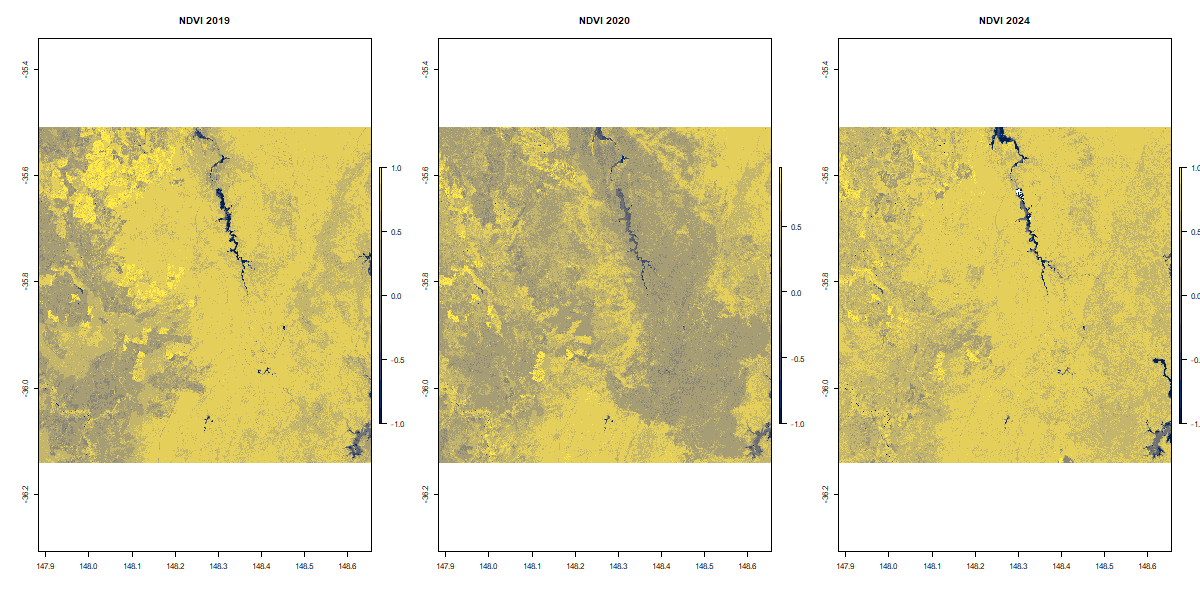
\includegraphics[width=\textwidth]{NDVI.png}
\end{columns}
\end{frame}

\begin{frame}[fragile]{\textbf{Differenze NDVI}}
\begin{lstlisting}
# Visualizzazione delle differenze
par(mfrow = c(1, 2))
plot(NDVI_diff_2020, col = viridis(10), main = "Differenza NDVI 2020-2019")
plot(NDVI_diff_2024, col = viridis(10), main = "Differenza NDVI 2024-2020")
\end{lstlisting}
\end{frame}

\begin{frame}{\textbf{Differenze NDVI}}
\begin{columns}
    \column{1\textwidth}
    \centering
    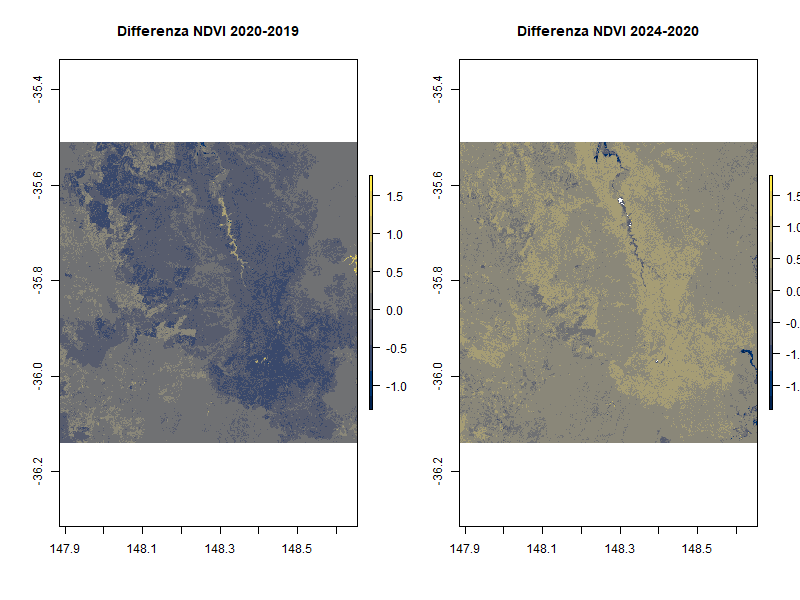
\includegraphics[width=\textwidth]{NDVI_diff.png}
\end{columns}
\end{frame}

\section{PCA (Analisi delle Componenti Principali)}

\begin{frame}[fragile]{\textbf{PCA (Analisi delle Componenti Principali)}}
\textbf{Obiettivo:} Identificare pattern principali nei valori NDVI.
\newline
\newline
\textbf{Procedura:}
\begin{lstlisting}
# PCA su 2019-2020
NDVI_stack_2019_2020 <- stack(NDVI_2019, NDVI_2020)
sample_pixels_2019_2020 <- sampleRandom(NDVI_stack_2019_2020, size = 10000)
PCA_2019_2020 <- prcomp(sample_pixels_2019_2020, scale. = TRUE)
summary(PCA_2019_2020)

# Proiezione
PCA_projection_2019_2020 <- predict(NDVI_stack_2019_2020, PCA_2019_2020, index = 1)
png("PCA_PC1_2019_2020.png", width = 800, height = 600)
plot(PCA_projection_2019_2020[[1]], main = "PC1 2019-2020", col = viridis(100))
dev.off()
\end{lstlisting}
\end{frame}

\begin{frame}{\textbf{PCA 2019-2020}}
\begin{columns}
    \column{0.5\textwidth}
    \centering
    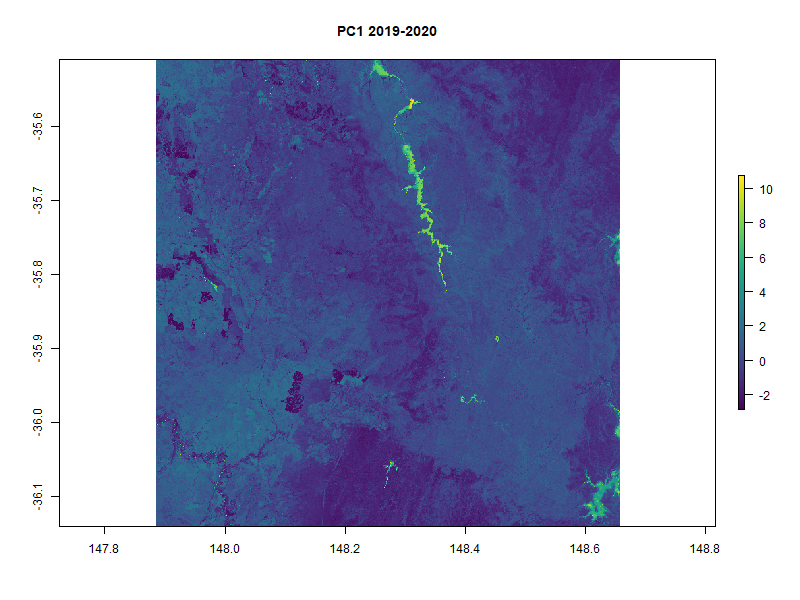
\includegraphics[width=\textwidth]{PCA_PC1_2019_2020.png}
    
    \column{0.5\textwidth}
    \centering
    \textbf{Summary della PCA}
    \begin{table}
        \centering
        \begin{tabular}{lcc}
            \toprule
            & PC1 \\
            \midrule
            Standard deviation     & 1.1177 \\
            Proportion of Variance & 0.6246 \\
            Cumulative Proportion  & 0.6246 \\
            \bottomrule
        \end{tabular}
    \end{table}
\end{columns}
\end{frame}

\begin{frame}[fragile]{\textbf{PCA (Analisi delle Componenti Principali)}}
\begin{lstlisting}
# PCA su 2020-2024
NDVI_stack_2020_2024 <- stack(NDVI_2020, NDVI_2024)
sample_pixels_2020_2024 <- sampleRandom(NDVI_stack_2020_2024, size = 10000)
PCA_2020_2024 <- prcomp(sample_pixels_2020_2024, scale. = TRUE)
summary(PCA_2020_2024)

# Proiezione
PCA_projection_2020_2024 <- predict(NDVI_stack_2020_2024, PCA_2020_2024, index = 1)
png("PCA_PC1_2020_2024.png", width = 800, height = 600)
plot(PCA_projection_2020_2024[[1]], main = "PC1 2020-2024", col = viridis(100))
dev.off()
\end{lstlisting}
\end{frame}

\begin{frame}{\textbf{PCA 2020-2024}}
\begin{columns}
    \column{0.5\textwidth}
    \centering
    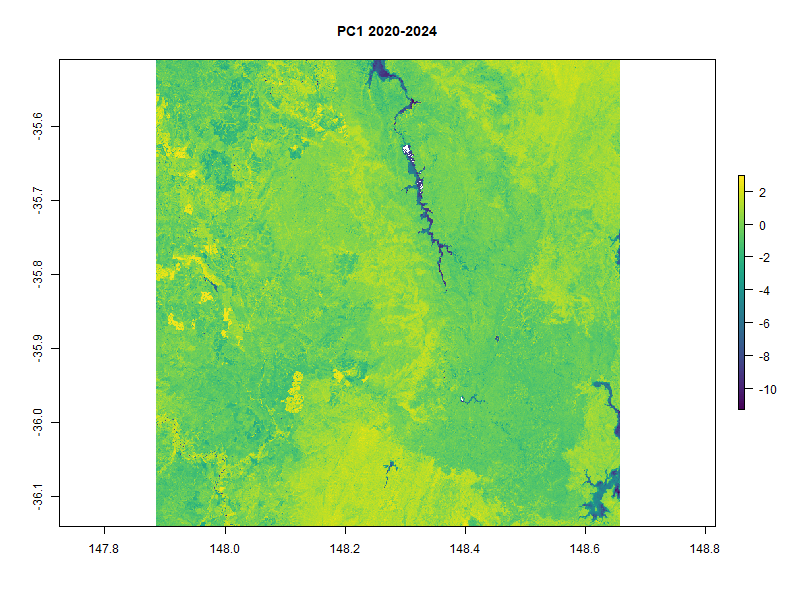
\includegraphics[width=\textwidth]{PCA_PC1_2020_2024.png}
    
    \column{0.5\textwidth}
    \centering
    \textbf{Summary della PCA}
    \begin{table}
        \centering
        \begin{tabular}{lcc}
            \toprule
            & PC1 \\
            \midrule
            Standard deviation     & 1.1825 \\
            Proportion of Variance & 0.6992 \\
            Cumulative Proportion  & 0.6992 \\
            \bottomrule
        \end{tabular}
    \end{table}
\end{columns}
\end{frame}

\section{Classificazione Land Cover}

\begin{frame}[fragile]{\textbf{Classificazione Land Cover}}
\textbf{Metodo:} K-Means clustering su immagini raster.
\newline
\newline
\textbf{Risultati per il 2019:}
\begin{lstlisting}
# Estrazione dei valori per il 2019
single_nr_2019 <- getValues(img_2019)
# Classificazione in tre cluster
k_cluster_2019 <- kmeans(single_nr_2019, centers = 3)
# Creazione immagine classificata
img_2019_class <- setValues(img_2019[[1]], k_cluster_2019$cluster)
# Visualizzazione
plot(img_2019_class, col = plasma(3), main = "Classificazione Land Cover 2019")
\end{lstlisting}
Simile per 2020 e 2024.
\end{frame}

\begin{frame}{\textbf{Immagini Classificazione Land Cover}}
\begin{columns}
    \column{0.33\textwidth}
    \centering
    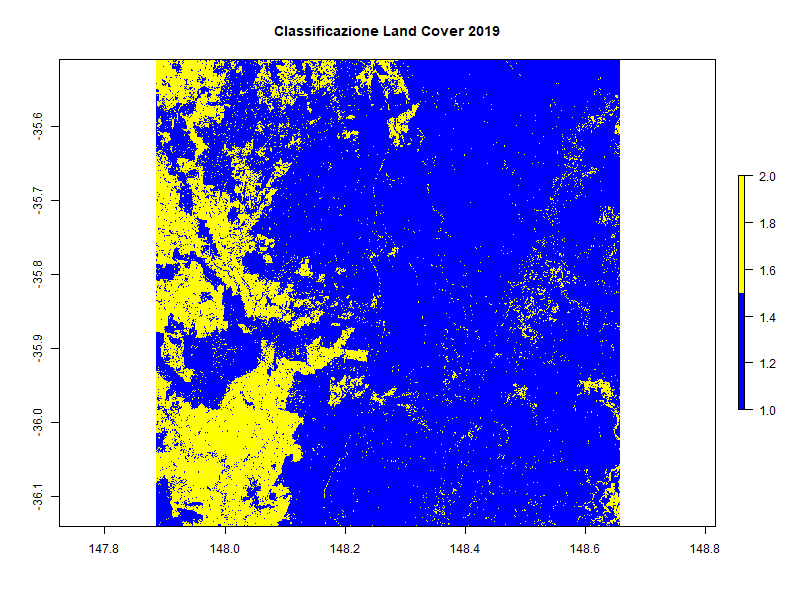
\includegraphics[width=\textwidth]{Land_Cover_2019.png}
    
    \column{0.33\textwidth}
    \centering
    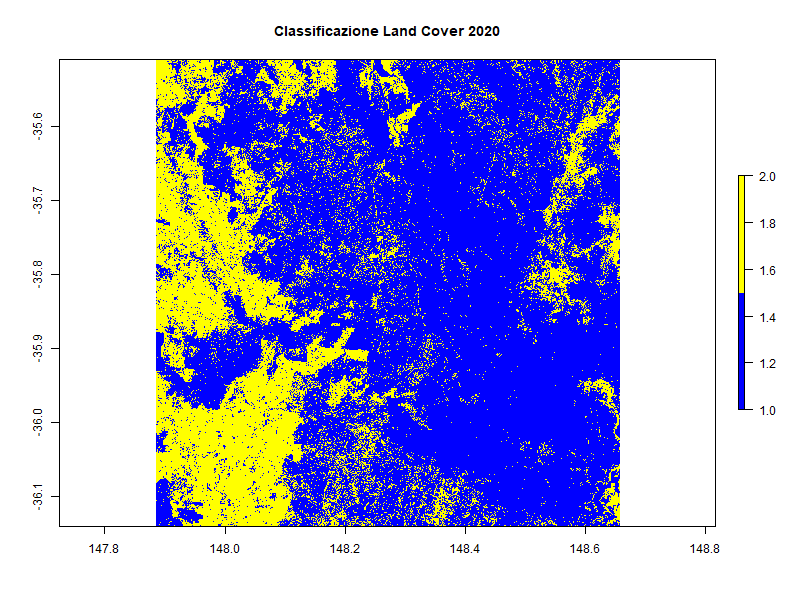
\includegraphics[width=\textwidth]{Land_Cover_2020.png}
    
    \column{0.33\textwidth}
    \centering
    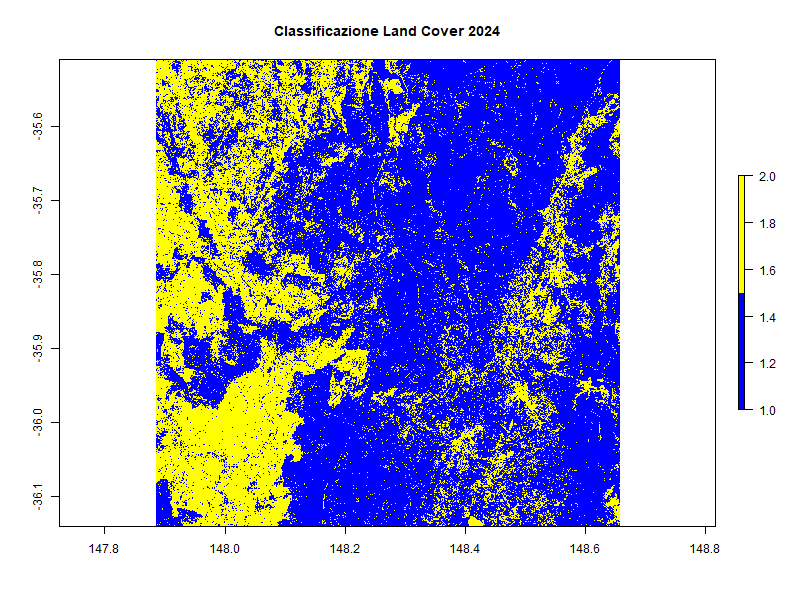
\includegraphics[width=\textwidth]{Land_Cover_2024.png}
\end{columns}
\end{frame}

\section{Confronto Copertura Vegetale}

\begin{frame}[fragile]{\textbf{Confronto Copertura Vegetale}}
\textbf{Percentuali di copertura vegetale:}
\begin{lstlisting}
copertura_vegetale <- c("buona", "ridotta", "assente")
# Supponendo che P_2019, P_2020, P_2024 siano definiti
Land_cover_perc <- data.frame(copertura_vegetale, P_2019, P_2020, P_2024)
\end{lstlisting}

\begin{columns}
    \column{0.33\textwidth}
    \centering
    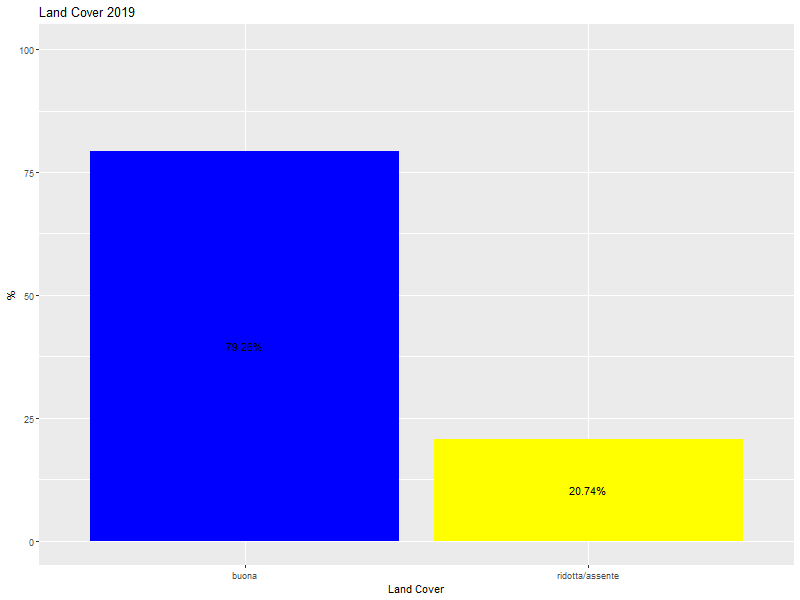
\includegraphics[width=\textwidth]{Percentuali_Land_Cover_2019.png}
    
    \column{0.33\textwidth}
    \centering
    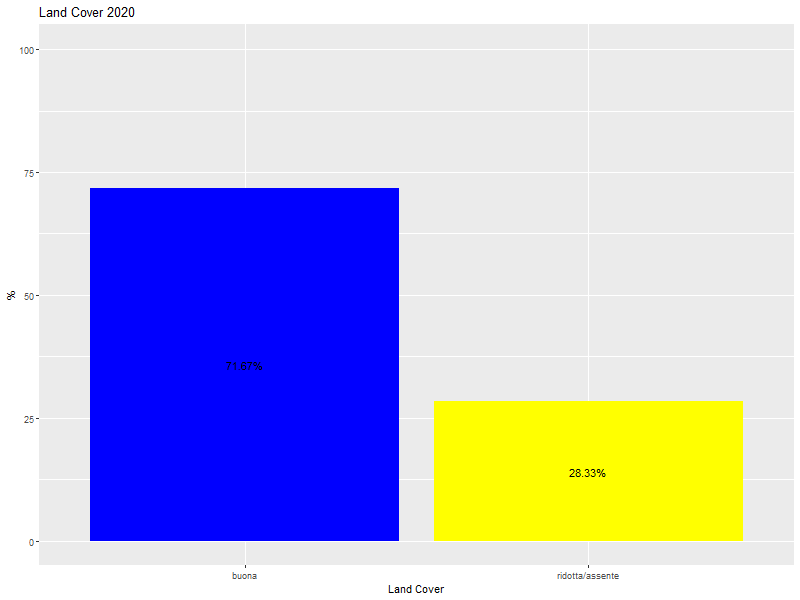
\includegraphics[width=\textwidth]{Percentuali_Land_Cover_2020.png}
    
    \column{0.33\textwidth}
    \centering
    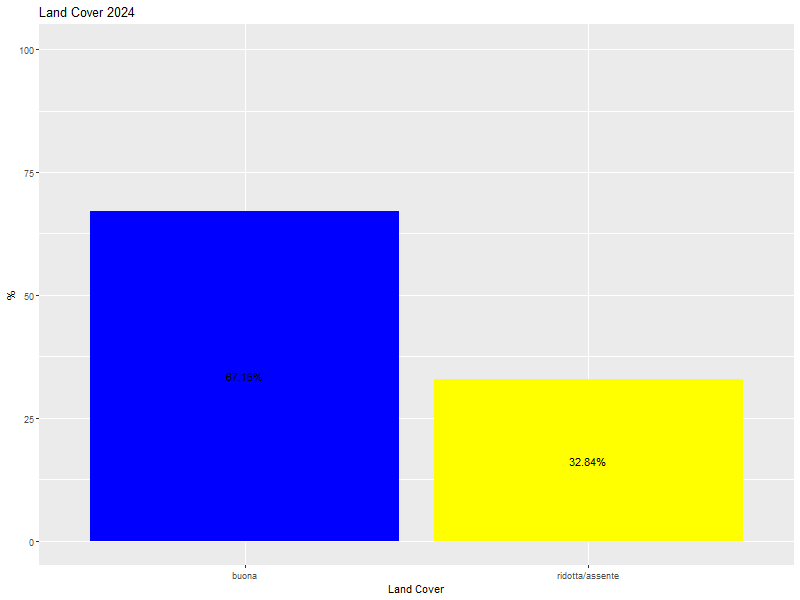
\includegraphics[width=\textwidth]{Percentuali_Land_Cover_2024.png}
\end{columns}
\end{frame}

\section{Conclusioni}

\begin{frame}{\textbf{Conclusioni}}
\begin{itemize}
    \item Gli incendi del 2019 hanno ridotto significativamente la copertura vegetale.
    \item Nel 2020, la copertura vegetale ha subito ulteriori danni.
    \item Nel 2024, si osserva una lenta ripresa con un aumento delle zone a ridotta vegetazione e una diminuzione di quelle a vegetazione assente.
\end{itemize}
\end{frame}

\section{Studi Futuri}

\begin{frame}{\textbf{Studi Futuri}}
\begin{itemize}
    \item Aggiunta di ulteriori anni per un'analisi più dettagliata.
    \item Studio della biodiversità e correlazioni con i dati satellitari.
    \item Analisi dell'efficacia degli interventi di ripristino.
\end{itemize}
\end{frame}

\begin{frame}{}
\centering
\textbf{Grazie per l'attenzione!}
\end{frame}

\end{document}
